\documentclass[11pt]{article}

\pdfinfoomitdate=1
\pdftrailerid{}
\pdfsuppressptexinfo=15

\usepackage[margin=1in]{geometry}
\usepackage{booktabs}
\usepackage{graphicx}
\usepackage{longtable}
\usepackage{tabularx}
\usepackage{array}
\usepackage{enumitem}
\usepackage{amsmath}
\usepackage[hidelinks,hypertexnames=false]{hyperref}
\usepackage{natbib}
\usepackage{setspace}
\usepackage{float}
\usepackage{url}
\graphicspath{{figures/}}
\hypersetup{
  pdftitle={Online Supplement: How Large Language Model Benchmarks Are Built},
  pdfauthor={Preston Botter},
  pdfsubject={Supplemental methods, results, and reproducibility materials for IRT-Viz-Eval},
  pdfkeywords={large language models, benchmark design, validity, psychological measurement, item response theory}
}
\setlist{leftmargin=*}
\onehalfspacing
\renewcommand{\thetable}{S\arabic{table}}
\renewcommand{\thefigure}{S\arabic{figure}}
\renewcommand{\theHtable}{supp.\arabic{table}}
\renewcommand{\theHfigure}{supp.\arabic{figure}}
\newcolumntype{Y}{>{\raggedright\arraybackslash}X}
\newcolumntype{Z}{>{\centering\arraybackslash}X}
\sloppy
\setlength{\tabcolsep}{3pt}

\title{Online Supplement\par\large How Large Language Model Benchmarks Are Built}
\author{Preston Botter\\
\small Indiana University Bloomington\\
\small \texttt{pdbotter@gmail.com}}
\date{August 2026}

\begin{document}
\maketitle

\section{Purpose and scope}

This supplement documents the benchmark-development decisions, empirical administration records, scoring rules, additional results, and reproducibility materials for the accompanying manuscript. It is intentionally more operational than the main article. The manuscript's purpose is to explain how an LLM benchmark is built and administered for a social-science audience. This supplement should not be read as evidence that IRT-Viz-Eval is already a validated psychometric scale for AI systems. It supplies the materials needed to inspect, reproduce, extend, and eventually validate the benchmark.

The benchmark is an instrumented evaluation procedure: a frozen task form, an elicitation contract, a configured model route, a response record, a deterministic scorer, and an aggregation rule. Its empirical scores describe these model-route-task configurations. They are not estimates of a human-like latent ability parameter, and the present study does not claim measurement invariance, generalizability across providers, or suitability for unsupervised psychometric work.

\section{Human assessment and LLM benchmark design}

\begin{table}[H]
\centering
\caption{Practical differences between assessments of people and benchmarks of LLM systems.}
\label{tab:supp-differences}
\begin{tabularx}{\linewidth}{p{0.18\linewidth}p{0.38\linewidth}p{0.38\linewidth}}
\toprule
Design issue & Educational or psychological assessment & LLM benchmark \\
\midrule
Object & Person, group, or population & Versioned model system under a specified interface \\
Administration & Instructions, timing, setting, accommodations & Prompt, context examples, media preprocessing, tools, decoding, retries \\
Response & Selected or constructed human performance & Generated tokens, tool calls, refusals, latency, malformed outputs \\
Exposure threat & Item security, coaching, practice & Pretraining, fine-tuning, evaluation leakage, public prompt reuse \\
Scoring & Key, rubric, rater, measurement model & Parser, executable check, metric, human rater, or model judge \\
Repeatability & Affected by persons and occasions & Also affected by sampling seeds and silent model updates \\
Typical claim & Standing on a construct or expected performance & Performance on a sampled task distribution under tested conditions \\
Lifecycle & Forms are revised and revalidated & Public tasks can saturate or contaminate quickly; versions may drift \\
\bottomrule
\end{tabularx}
\end{table}

\section{Study and release manifest}

The frozen release contains 14 base mathematical stimuli, six rendering profiles, 84 image-level stimuli, and 198 scored tasks. The number of tasks varies by image because different curve families support different observable questions. Every model received the same 198 task identifiers and native PNG images. The benchmark generator, task records, ground-truth values, image files, scoring code, schemas, prompts, and analysis scripts are included in the accompanying reproducibility archive and at \url{https://github.com/pbotter42/IRT-Viz-Eval}.

\begin{table}[H]
\centering
\caption{Core study objects and their roles.}
\begin{tabularx}{\linewidth}{p{0.23\linewidth}p{0.71\linewidth}}
\toprule
Object & Role in benchmark development \\
\midrule
Base stimulus & Mathematical object with stored parameters, curve family, and exact ground truth. \\
Rendering profile & Meaning-preserving visual transformation used to probe presentation robustness. \\
Image-level stimulus & One base stimulus rendered under one profile and linked to an image file. \\
Task & One elicitation and scoring contract attached to an image-level stimulus. \\
Response & One model output under a named route, with raw output, latency, tokens, and provenance. \\
Judgment & Deterministic field-level scoring record retaining errors, rationale points, totals, and normalization. \\
\bottomrule
\end{tabularx}
\end{table}

\section{Model administration and provenance}

All five complete runs used Hugging Face Inference Providers as the common API route. The compute provider was recorded in the requested model string. This improves interface comparability while preserving provider differences as part of the observed system. A direct OpenAI or Gemini adapter can be used in future work, but a consumer ChatGPT or Gemini subscription is not itself a reproducible API administration condition.

\subsection{API and deployment options}

\begin{table}[H]
\centering
\small
\caption{API and deployment options for administering a multimodal benchmark.}
\label{tab:supp-api-options}
\begin{tabularx}{\linewidth}{p{0.17\linewidth}p{0.22\linewidth}p{0.27\linewidth}p{0.27\linewidth}}
\toprule
Route & Examples & Primary advantage & Measurement concern \\
\midrule
Direct vendor API & OpenAI Responses; Google Gemini & Native model controls and provider metadata & Separate credentials, billing, schemas, and version policies \\
Model router or hub & Hugging Face Inference Providers & One task adapter can reach several model families & Routing and underlying compute provider must be recorded \\
Dedicated endpoint & Managed cloud or Hugging Face endpoint & Stable deployment and configurable resources & Setup cost and endpoint configuration become part of the system \\
Local inference & Transformers, vLLM, or similar runtime & Control over weights, decoding, and logs & Hardware, quantization, runtime, and preprocessing affect comparability \\
\bottomrule
\end{tabularx}
\end{table}

\begin{table}[H]
\centering
\scriptsize
\caption{Overall results for all complete administrations.}
\label{tab:supp-overall}
\begin{tabular}{p{0.22\linewidth}cccccc}
\toprule
Model & $n$ & Mean & 95\% CI & Points & Empty & Median latency \\
\midrule
Qwen2.5-VL 72B & 198 & .719 & [.656, .788] & 905/1236 & 0.0\% & 3.48 s \\
Qwen3-VL 30B & 198 & .704 & [.643, .774] & 873/1236 & 0.0\% & 2.25 s \\
GLM-4.5V & 198 & .628 & [.536, .727] & 668/1236 & 16.7\% & 13.79 s \\
Gemma 3 4B & 198 & .629 & [.587, .673] & 742/1236 & 0.0\% & 2.14 s \\
Gemma 3 12B & 198 & .600 & [.549, .653] & 782/1236 & 0.0\% & 3.04 s \\
\bottomrule
\end{tabular}
\end{table}

\begin{table}[H]
\centering
\scriptsize
\caption{Administration and output-format diagnostics.}
\label{tab:supp-admin}
\begin{tabular}{p{0.17\linewidth}p{0.27\linewidth}p{0.24\linewidth}ccc}
\toprule
Model & Requested route & Returned identifier & Nonempty & Parseable & Tokens \\
\midrule
Qwen2.5-VL 72B & Qwen/Qwen2.5-VL-72B-Instruct:ovhcloud & Qwen2.5-VL-72B-Instruct & 198/198 & 198/198 & 219,565 \\
Qwen3-VL 30B & Qwen/Qwen3-VL-30B-A3B-Instruct:novita & qwen/qwen3-vl-30b-a3b-instruct & 198/198 & 194/198 & 189,730 \\
GLM-4.5V & zai-org/GLM-4.5V:novita & zai-org/glm-4.5v & 165/198 & 152/198 & 342,107 \\
Gemma 3 4B & google/gemma-3-4b-it:deepinfra & google/gemma-3-4b-it & 198/198 & 198/198 & 85,531 \\
Gemma 3 12B & google/gemma-3-12b-it:deepinfra & google/gemma-3-12b-it & 198/198 & 198/198 & 84,523 \\
\bottomrule
\end{tabular}
\end{table}

\begin{table}[H]
\centering
\scriptsize
\caption{Task-type results for every complete model run.}
\label{tab:supp-task}
\begin{tabular}{p{0.24\linewidth}cccccc}
\toprule
Task type & $n$ & Qwen2.5-VL 72B & Qwen3-VL 30B & GLM-4.5V & Gemma 3 4B & Gemma 3 12B \\
\midrule
Model identification & 84 & .611 & .730 & .639 & .698 & .583 \\
Parameter estimation & 24 & .597 & .642 & .147 & .533 & .675 \\
Probability at theta=0 & 30 & .800 & .433 & .873 & .567 & .413 \\
Information peak & 30 & .979 & .950 & .946 & .721 & .850 \\
Category-curve reasoning & 18 & .646 & .597 & .125 & .444 & .472 \\
Test expected score & 6 & 1.000 & .833 & .833 & .361 & .361 \\
Non-monotonic peak & 6 & .963 & .907 & .889 & .722 & .833 \\
\bottomrule
\end{tabular}
\end{table}

\begin{table}[H]
\centering
\scriptsize
\caption{Curve-family results for every complete model run.}
\label{tab:supp-family}
\begin{tabular}{p{0.24\linewidth}cccccc}
\toprule
Curve family & $n$ & Qwen2.5-VL 72B & Qwen3-VL 30B & GLM-4.5V & Gemma 3 4B & Gemma 3 12B \\
\midrule
Dichotomous ICC & 72 & .619 & .602 & .506 & .603 & .552 \\
Item information & 48 & .867 & .849 & .841 & .740 & .732 \\
Polytomous curves & 36 & .656 & .688 & .424 & .546 & .551 \\
Test characteristic & 12 & .722 & .750 & .694 & .514 & .403 \\
Test information & 12 & .813 & .813 & .750 & .677 & .698 \\
Unfolding & 18 & .788 & .658 & .833 & .652 & .604 \\
\bottomrule
\end{tabular}
\end{table}

\begin{table}[H]
\centering
\scriptsize
\caption{Rendering-profile results for every complete model run.}
\label{tab:supp-style}
\begin{tabular}{p{0.28\linewidth}ccccc}
\toprule
Rendering profile & Qwen2.5-VL 72B & Qwen3-VL 30B & GLM-4.5V & Gemma 3 4B & Gemma 3 12B \\
\midrule
Matplotlib light & .709 & .729 & .599 & .666 & .593 \\
Seaborn white-grid & .721 & .709 & .646 & .643 & .584 \\
ggplot gray & .746 & .700 & .630 & .608 & .627 \\
Grayscale & .717 & .692 & .611 & .627 & .597 \\
Dark high-contrast & .736 & .683 & .619 & .611 & .555 \\
Lattice-like & .687 & .712 & .663 & .621 & .644 \\
\bottomrule
\end{tabular}
\end{table}

\begin{table}[H]
\centering
\scriptsize
\caption{All paired cluster-bootstrap differences (row model minus column model).}
\label{tab:supp-pairs}
\begin{tabular}{p{0.24\linewidth}p{0.24\linewidth}cc}
\toprule
Model A & Model B & Difference & 95\% CI \\
\midrule
GLM-4.5V & Gemma 3 4B & -0.001 & [-0.078, .076] \\
GLM-4.5V & Gemma 3 12B & .028 & [-0.054, .113] \\
GLM-4.5V & Qwen3-VL 30B & -0.076 & [-0.142, -0.008] \\
GLM-4.5V & Qwen2.5-VL 72B & -0.091 & [-0.145, -0.039] \\
Gemma 3 4B & Gemma 3 12B & .029 & [-0.004, .056] \\
Gemma 3 4B & Qwen3-VL 30B & -0.075 & [-0.141, -0.021] \\
Gemma 3 4B & Qwen2.5-VL 72B & -0.090 & [-0.145, -0.041] \\
Gemma 3 12B & Qwen3-VL 30B & -0.104 & [-0.172, -0.047] \\
Gemma 3 12B & Qwen2.5-VL 72B & -0.120 & [-0.179, -0.066] \\
Qwen3-VL 30B & Qwen2.5-VL 72B & -0.015 & [-0.042, .008] \\
\bottomrule
\end{tabular}
\end{table}


The first GLM response file contained 199 raw rows because one response identifier was duplicated during resumable collection. The preparation script retained one completed record per response identifier, removed the duplicate, and required exactly one unique record for each of the 198 task identifiers. All other complete files contained 198 raw rows and 198 unique tasks. No API-error rows remained in the complete files used for scoring.

\section{Diagnostic baseline profiles}

The oracle, noisy, and blind baselines test whether the benchmark pipeline distinguishes exact, approximate, and weak responses. They do not estimate model performance or establish content validity. Figure~\ref{fig:supp-validation} displays overall and task-family separation.

\begin{figure}[H]
\centering
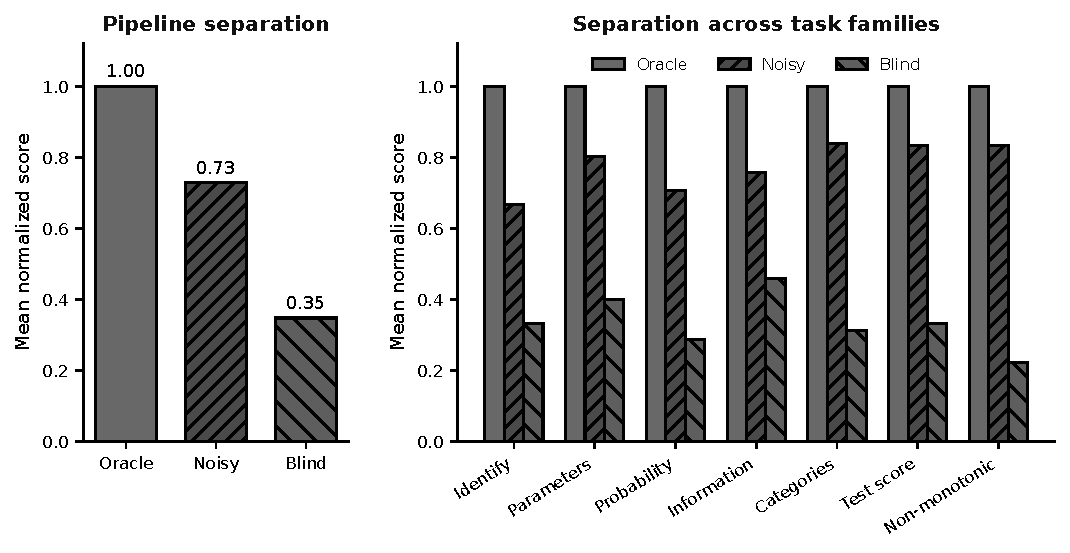
\includegraphics[width=\linewidth]{validation_profiles.pdf}
\caption{Diagnostic pipeline validation. The left panel shows overall separation of the oracle, noisy, and blind baselines; the right panel shows separation by task family. Because these are constructed local baselines, the graph validates benchmark mechanics only.}
\label{fig:supp-validation}
\end{figure}

\section{Rendering and curve-family profiles}

Figure~\ref{fig:supp-robustness} disaggregates scores by rendering profile and curve family. The style panels probe controlled presentation changes, whereas the curve-family panels describe substantive content differences.

\begin{figure}[H]
\centering
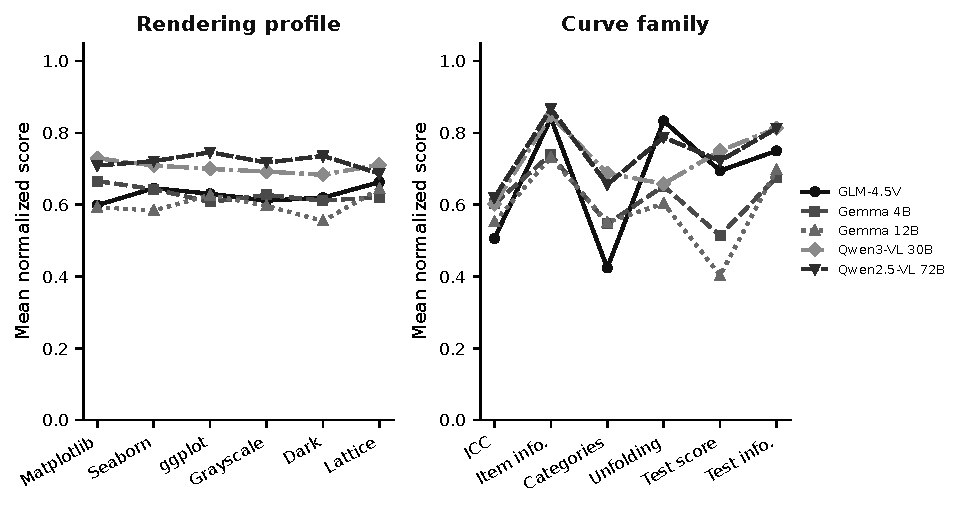
\includegraphics[width=\linewidth]{empirical_robustness_profiles.pdf}
\caption{Mean task-normalized scores by rendering profile and curve family. Similar style ranges coexist with larger content-profile differences, illustrating why both nuisance-condition and substantive-domain disaggregation are needed.}
\label{fig:supp-robustness}
\end{figure}

\section{Frozen elicitation contract}

The task prompt is generated from the task record. It supplies the model with one PNG image and a task-specific request. The prompt asks for JSON containing the expected fields and a short visual rationale. The task record, rather than an undocumented conversational instruction, is the source of the requested fields and scoring thresholds.

The model-visible administration contract is:

\begin{enumerate}
\item one native benchmark PNG image;
\item one zero-shot task prompt with no demonstrations;
\item no external tools, retrieval, or browsing;
\item a maximum completion length of 1,200 tokens;
\item one response per task in the reported administration;
\item raw output retained before parsing;
\item task-specific JSON fields plus a short rationale;
\item deterministic scoring after collection, with no LLM-as-a-judge.
\end{enumerate}

Provider defaults were not fully harmonized. Temperature, image-token accounting, reasoning-token accounting, hidden serving details, and throughput can differ. The correct interpretation is therefore performance of each named model route under the frozen task and prompt contract, not a claim that model weights alone caused every observed difference.

\section{Scoring and missing-output rules}

Categorical and integer fields receive exact-match credit after conservative normalization. Numeric fields receive graded credit under task-specific absolute-error bands. For common parameter fields, errors within 0.15, 0.30, and 0.50 receive 3, 2, and 1 points; larger errors receive 0. Probability fields use tighter bands of 0.05, 0.10, and 0.20. The rationale component awards zero to two points using a fixed rule based on prespecified psychometric terms and minimum explanatory content. It is a reproducible proxy for visible rationale evidence, not a semantic judgment of whether a model's complete explanation is correct.

For each task, the total is divided by the maximum available points for that task. The primary model score is the unweighted mean of these 198 task-normalized scores. This makes each task contribute equally even though tasks request different numbers of fields. Raw point totals are retained as a sensitivity analysis because they weight multi-field tasks more heavily.

Empty outputs, API-error outputs, malformed JSON, missing requested fields, and unparsable values remain in the response and judgment files. A missing or invalid field receives zero for that field; it is not silently removed from the denominator. The main paper reports empty-output and parseable-output rates separately because they describe operational behavior that a score alone can hide.

\section{Uncertainty and analysis decisions}

The primary uncertainty interval is a 95\% cluster bootstrap over the 14 base stimuli. For each draw, base-stimulus clusters are sampled with replacement and all linked tasks within each sampled cluster are retained. This accounts for the fact that six rendering profiles and multiple task records are not independent replications of mathematical content. Pairwise intervals resample the same clusters after aligning model judgments by task identifier.

The cluster bootstrap does not represent within-model sampling variability, because the study collected one response per task. It also does not represent provider drift, future model updates, judge uncertainty, or uncertainty in the deterministic rubric. These are separate validation targets. The supplement therefore reports descriptive intervals without converting them into general claims about stable model rankings.

\section{Additional interpretation guidance}

The results can support several bounded statements: the named routes produced different levels of performance on this task distribution; Qwen2.5-VL 72B and Qwen3-VL 30B had the highest observed aggregate scores; task profiles differed; and output validity and latency differed materially. The results cannot support the statements that one model has a general intelligence level, that the benchmark is invariant across providers, that success on synthetic plots transfers to operational psychometric practice, or that a model is safe for unsupervised assessment decisions.

This distinction mirrors a central lesson from educational and psychological measurement: scores acquire meaning through design, evidence, and intended use. In this project, that lesson is used to improve benchmark construction. The paper is not claiming that a benchmark total becomes a validated AI psychometric scale merely because it has an item matrix, a rubric, or an IRT-related content domain.

\section{Recommended expert-validation study}

The next study should obtain independent content and response-process evidence. A practical design is:

\begin{enumerate}
\item recruit psychometricians or advanced measurement students to review the capability map and content matrix;
\item ask experts to classify a stratified sample of images by curve family, visual feature, and intended task;
\item collect blinded expert scores for model responses, including partial credit and rationale quality;
\item estimate agreement between the deterministic rubric and expert scoring at the field level;
\item repeat a subset of model calls under the same prompt to estimate within-route stochasticity;
\item counterbalance prompt wording, answer-field order, and output format as explicit administration facets;
\item add empirical plots with estimation noise, confidence bands, dense overlays, truncated axes, and accessibility constraints;
\item compare benchmark performance with a separate authentic psychometric-review task, without treating that correlation as automatic proof of construct validity.
\end{enumerate}

This design would add evidence about content representation, response processes, relations to an external task, and consequences. It would still require a separate argument before the score could be used for operational decisions.

\section{Repository map and reproduction}

The following files are the core reproducibility objects:

\begin{table}[H]
\centering
\scriptsize
\caption{Repository map and contents.}
\label{tab:supp-repository-map}
\begin{tabular}{p{0.43\linewidth}p{0.49\linewidth}}
\toprule
Path & Contents \\
\midrule
\texttt{data/benchmark/stimuli.jsonl} & Stimulus records, parameters, ground truth, and visual metadata. \\
\texttt{data/benchmark/tasks.jsonl} & Task prompts, expected fields, thresholds, and image links. \\
\texttt{data/benchmark/images/} & PNG files shown to models. \\
\texttt{data/empirical/} & Deduplicated model response records used for analysis. \\
\texttt{paper/prepare\_empirical\_results.py} & Deduplication, scoring, uncertainty, and result-table preparation. \\
\texttt{paper/generate\_figures.py} & Reproducible generation of all main-paper figures. \\
\texttt{paper/generate\_supplement.py} & Reproducible generation of supplemental empirical tables. \\
\texttt{tests/} & Unit tests for generation, schemas, scoring, and provider behavior. \\
\bottomrule
\end{tabular}
\end{table}

After dependencies are installed, the empirical tables and figures can be regenerated with:

\begin{verbatim}
PYTHONPATH=src python3 \
  paper/prepare_empirical_results.py
PYTHONPATH=src python3 \
  paper/generate_supplement.py
PYTHONPATH=src python3 \
  paper/generate_figures.py --grayscale \
  --output-dir paper/figures_grayscale
\end{verbatim}

A new provider administration should first use a small pilot, preserve the exact requested model and provider string, and write to a new JSONL path. A full run should use the same output path when resumed so successful response identifiers can be skipped. API keys must be supplied through the local environment or Hugging Face credential store and must never be committed.

\section{Supplemental reporting checklist}

Before releasing a new benchmark version, record: the intended use; the exact model object; capability definitions; content and exclusion rules; task and image generators; ground-truth derivation; prompt and output schema; provider and access date; timeout and retry policy; raw output retention; parser and scorer versions; missing-output handling; uncertainty procedure; human or model-judge provenance if applicable; contamination risks; licenses; version changes; maintenance owner; and unsupported interpretations.

\end{document}
